
\chapter{Aufgabe D10}


Die \autoref{fig:RandomGenerator} zeigt den \glqq Random Number Generator"' umgesetzt in ASCET.

\begin{figure}[h!]
	\centering
	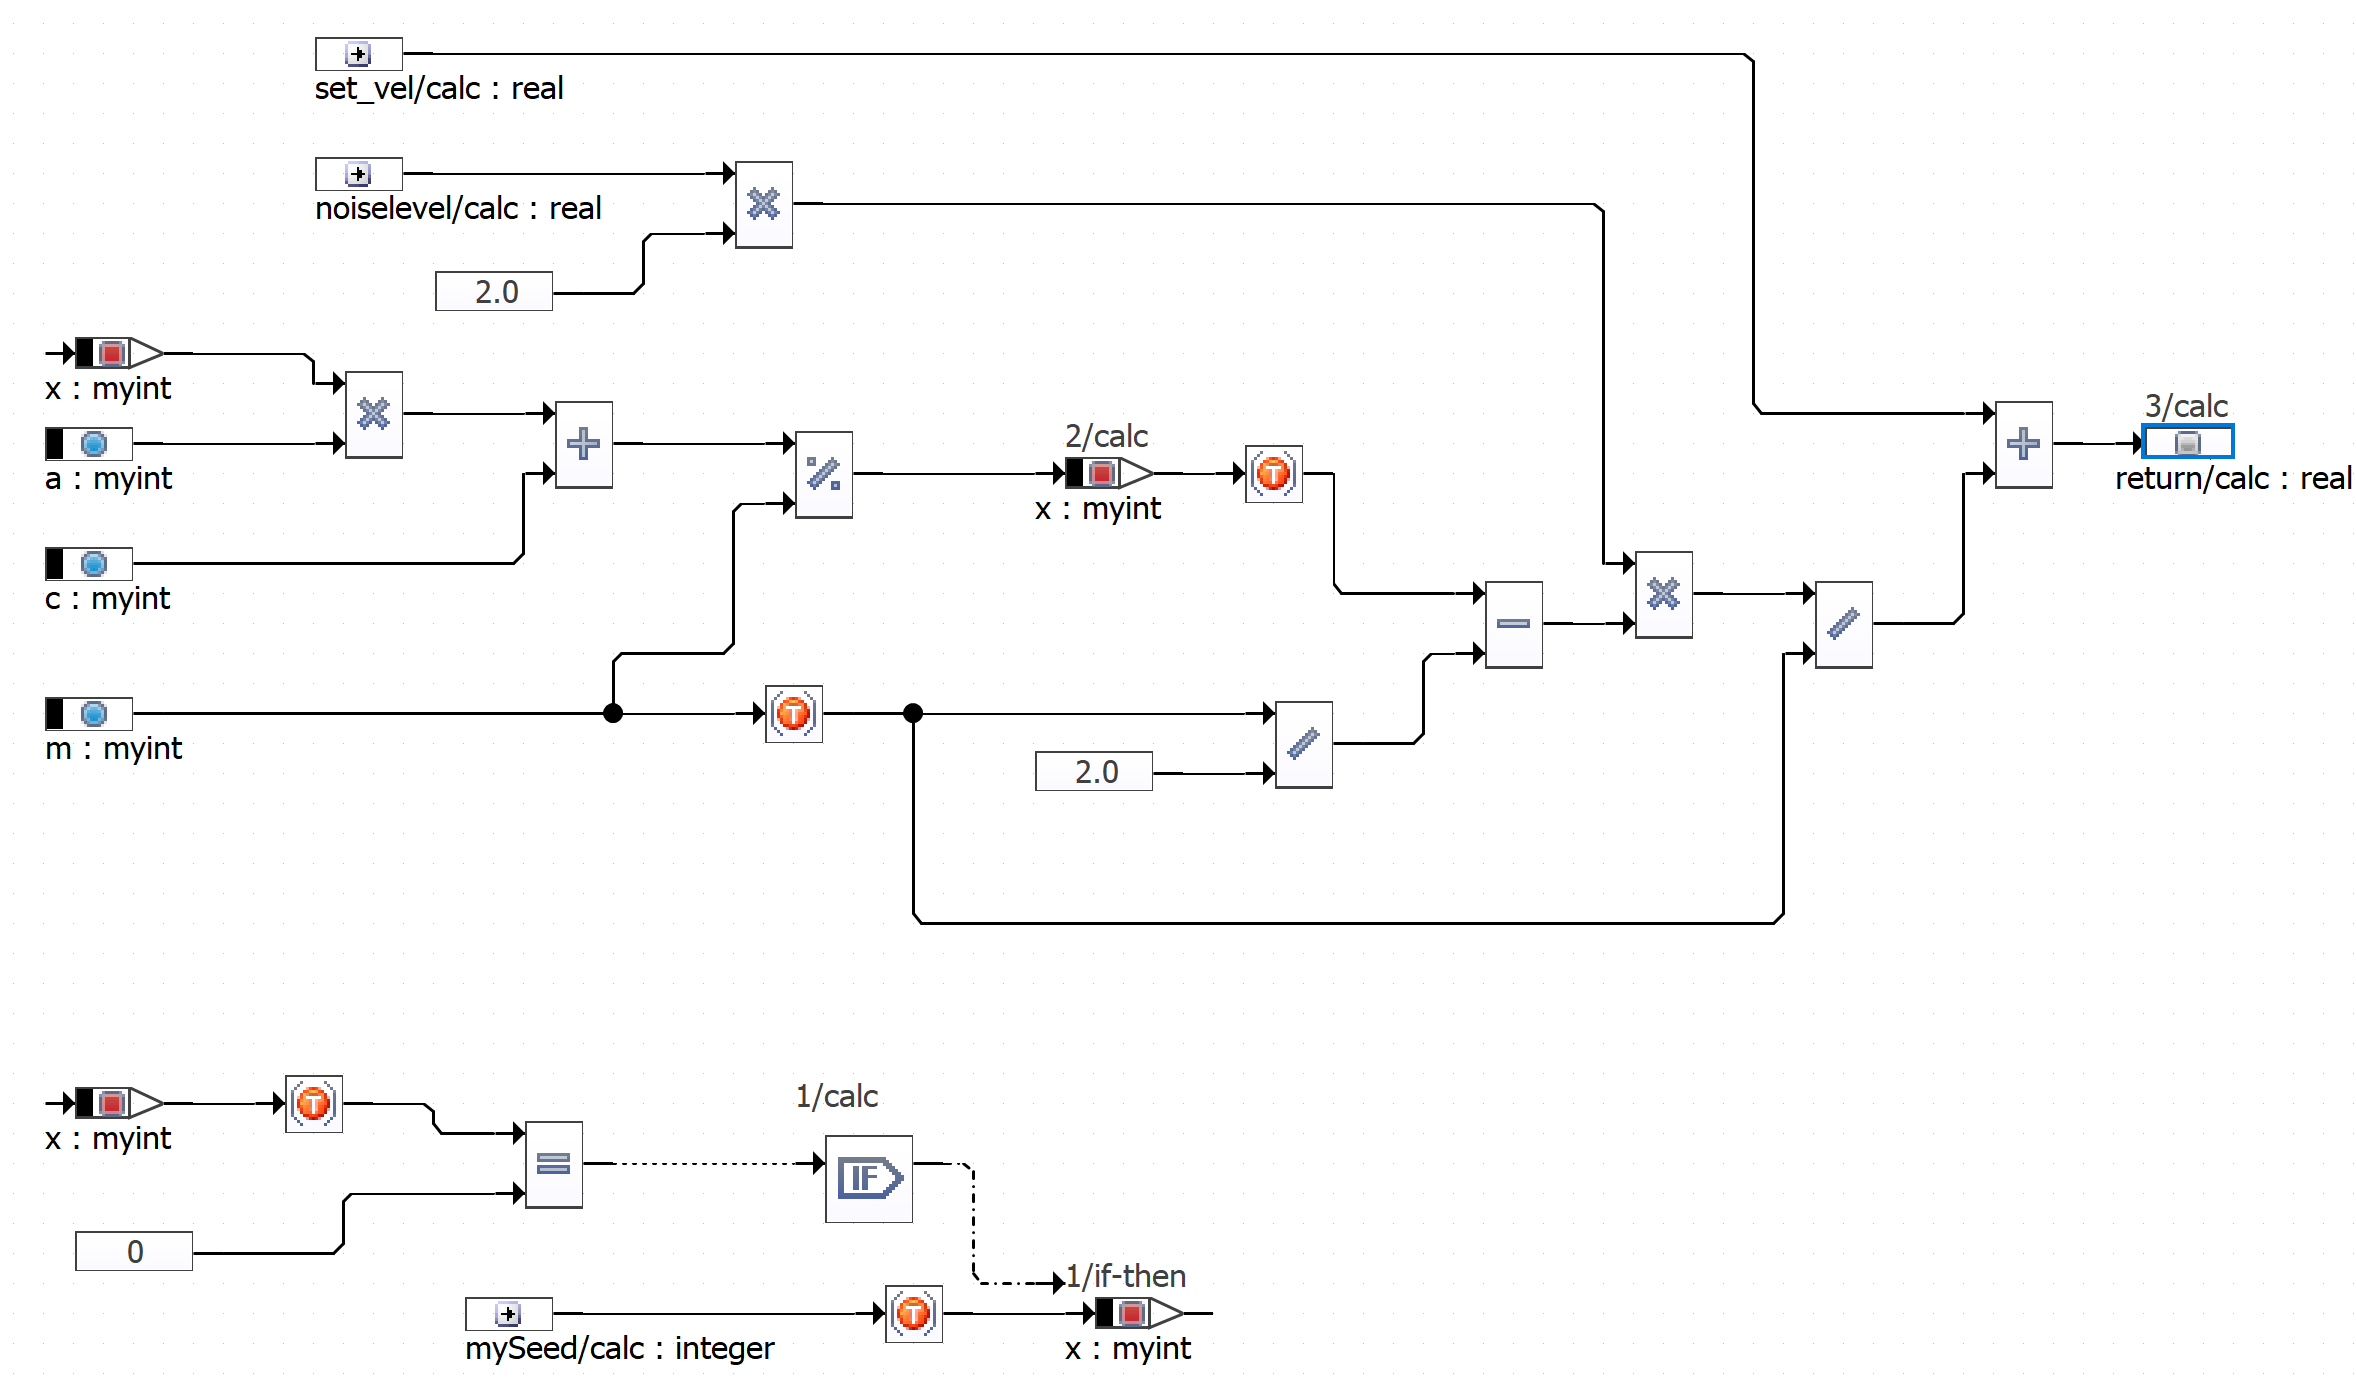
\includegraphics[width=1\linewidth]{../Graphiken/RandomGenerator.png}
	\caption{Random Number Generator}
	\label{fig:RandomGenerator}
\end{figure}

Der Code des Unittests für den \glqq Random Number Generator"' wird im Folgenden dargestellt.

\begin{lstlisting}
package components;
import assertLib.Assert;
static class RandomGeneratorTest {
	
	RandomGenerator rg;
	RingBuffer rb;
	
	@Test
	public void testcalc() {
		real set_vel = 100.0;
		real noiselevel = 5.0;
		integer mySeed = 10;
		real erg = rg.calc(set_vel, noiselevel, mySeed);
		Assert.assertNear(erg, 96.1425781, 0.01);
	}
	
	@Test
	public void testcalc2() {
		real set_vel = 100.0;
		real noiselevel = 5.0;
		integer mySeed = 10;
		for(i in 0 .. 99){
			real erg = rg.calc(set_vel, noiselevel, mySeed);
			rb.put(erg);
			for(j in 1 .. 999){
				real act = rb.getIndex(0);
				Assert.assertNotEqual(act, rb.getIndex(j));
			}
		}
	}
}
\end{lstlisting}